\chapter{Implementasi dan Pengujian}
\label{chap:implementasi dan pengujian}

Bab ini membahas tentang implementasi dan pengujian perangkat lunak berdasarkan rancangan yang sudah dibuat. Ada dua jenis pengujian yang dilakukan, yaitu pengujian fungsional dan pengujian eksperimental. Bab ini juga membahas tentang lingkungan yang digunakan untuk pengujian perangkat lunak ini.

\section{Lingkungan untuk Pengujian}
Pengujian fungsional dan pengujian eksperimental dilakukan menggunakan dua jenis lingkungan yang berbeda. 
\begin{enumerate}
	\item Pengujian Fungsional. \\
	Berikut spesifikasi perangkat keras dan perangkat lunak yang digunakan untuk melakukan pengujian fungsional
	\begin{table}[H] %atau h saja untuk "kira kira di sini" 
		\caption{Lingkungan perangkat keras untuk pengujian fungsional}
		\label{tab:lingkunganpkpf}
		\resizebox{\textwidth}{!}{%
			\begin{tabular}{|l|l|}
				\hline
				\textbf{Parameter} & \textbf{Nilai} \\
				\hline
				\textit{Processor} & \textit{Intel Core i5 4200u}\\
				\hline
				\textit{Graphics Processing Unit (GPU)} & \textit{Intel HD Graphics HD4000} dan \textit{Nvidia GeForce 840M}\\
				\hline
				\textit{Random Access Memory (RAM)}& 12.00GB DDR3\\
				\hline
				\textit{Storage} & 120GB \textit{SSD} dan 1TB \textit{Harddisk}\\
				\hline
		\end{tabular}}
	\end{table}

	\begin{table}[H] %atau h saja untuk "kira kira di sini" 
		\caption{Lingkungan perangkat lunak untuk pengujian fungsional}
		\label{tab:lingkunganplpf}
		\resizebox{\textwidth}{!}{%
			\begin{tabular}{|l|l|}
				\hline
				\textbf{Parameter} & \textbf{Nilai} \\
				\hline
				Sistem Operasi & Windows 10 \textit{10 Education 64-bit}\\
				\hline
				Bahasa Pemrograman & PHP, JavaScript, CSS dan HTML\\
				\hline
				\textit{Text Editor} & \textit{Atom}\\
				\hline
				\textit{Framework} & \textit{CodeIgniter}\\
				\hline
				\multirow{4}{*}{Perangkat Lunak pendukung} 	& \textit{XAMPP Control Panel} v3.2.2\\
															& \textit{Google Chrome Version} 65.0.3325.181 (Official Build) (64-bit)\\
															& \textit{Firefox Quantum} 59.0.2 (64-bit)\\
															& \textit{Microsoft Excel} 2016\\
				\hline
		\end{tabular}}
	\end{table}

	\item Pengujian Eksperimental. \\
	Berikut spesifikasi perangkat keras dan perangkat lunak yang digunakan untuk melakukan pengujian eksperimental
	\begin{table}[H] %atau h saja untuk "kira kira di sini" 
		\caption{Lingkungan perangkat keras untuk pengujian eksperimental}
		\centering
		\label{tab:lingkunganpkpe}
		%\resizebox{\textwidth}{!}
	\end{table}
	
	\begin{table}[h] %atau h saja untuk "kira kira di sini" 
		\caption{Lingkungan perangkat lunak untuk pengujian eksperimental}
		\label{tab:lingkunganplpe}
		\centering
		%\resizebox{\textwidth}{!}
	\end{table}
\end{enumerate}

\section{Implementasi}
Hasil implementasi dari rancangan perangkat lunak yang sudah dibuat ini terdiri dari tiga bagian, yaitu
\begin{enumerate}
	\item Kode program \\
	Perubahan dan penambahan kode program untuk mengimplementasi kebutuhan \textit{Sharif Judge}, ditulis dalam bahasa pemrograman PHP. Seluruh perubahan kode program telah dijabarkan dalam setiap sub bab pada bab 4. Kode program untuk halaman \textit{Logs} dan \textit{Hall of Fame} dapat dilihat di bab Lampiran --.
	\item Basis Data \\
	Terdapat penambahan \textit{key} dan \textit{value} dalam mengimplementasi kebutuhan \textit{Sharif Judge} pada sub bab 4.7. Pada tabel \textit{shj\_settings} ditambahkan \textit{shj\_key} dengan nama \textit{lock\_student\_display\_name} dan \textit{shj\_value} dengan nilai 0. Berikut struktur tabel \textit{shj\_settings}
	
	\begin{table}[H] %atau h saja untuk "kira kira di sini"
		\centering 
		\caption{Struktur Tabel \textit{shj\_settings}}
		\label{tab:atributtabelsettings}
		\resizebox{\textwidth}{!}{
		\begin{tabular}{|c|c|}
			\hline
			\textbf{shj\_key} & \textbf{shj\_value}\\
			\hline
			\textit{timezone} & Asia/Jakarta\\
			\hline
			\textit{tester\_path} & path{C:/xampp/htdocs/tester}\\
			\hline
			\textit{assignments\_root} & path{C:/xampp/htdocs/assignments}\\
			\hline
			\textit{file\_size\_limit} & 50\\
			\hline
			\textit{output\_size\_limit} & 1024\\
			\hline
			\textit{queue\_is\_working} & 0\\
			\hline
			\textit{default\_late\_rule} & /** Put coefficient (from 100) in variable \$co...\\
			\hline
			\textit{enable\_easysandbox} & 1\\
			\hline
			\textit{enable\_c\_shield} & 1\\
			\hline
			\textit{enable\_cpp\_shield} & 1\\
			\hline
			\textit{enable\_py2\_shield} & 1\\
			\hline
			\textit{enable\_py3\_shield} & 1\\
			\hline
			\textit{enable\_java\_policy} & 1\\
			\hline
			\textit{enable\_log} & 1\\
			\hline
			\textit{submit\_penalty} & 300\\
			\hline
			\textit{enable\_registration} & 1\\
			\hline
			\textit{registration\_code} & 0\\
			\hline
			\textit{mail\_from} & shj@example.com\\
			\hline
			\textit{mail\_from\_name} & \textit{Sharif Judge}\\
			\hline
			\textit{reset\_password\_mail} & <p> Someone requested a password reset for your S...\\
			\hline
			\textit{add\_user\_mail} & <p> Hello! You are registered in SharIF Judge at ...\\
			\hline
			\textit{moss\_userid} & \\
			\hline
			\textit{results\_per\_page\_all} & 40\\
			\hline
			\textit{results\_per\_page\_final} & 80\\
			\hline
			\textit{week\_start} & 0\\
			\hline
			\textit{lock\_student\_display\_name} & 1\\
			\hline
		\end{tabular}}
	\end{table}
	
	Terdapat penambahan atribut dalam mengimplementasi kebutuhan \textit{Sharif Judge} pada sub bab 4.8. Pada tabel \textit{shj\_assignments} ditambahkan atribut baru dengan nama \textit{archived\_assignment}. Berikut struktur tabel \textit{shj\_assignments}
	
	\begin{table}[H] %atau h saja untuk "kira kira di sini"
		\centering 
		\caption{Struktur Tabel \textit{shj\_assignments}}
		\label{tab:atributtabelassignments}
		%\resizebox{\textwidth}{!}{
		\begin{tabular}{|c|c|c|c|}
			\hline
			\textbf{Atribut} & \textbf{Tipe Data} & \textbf{Ukuran}  & \textbf{Default} \\
			\hline
			\textit{id (primary key)} & int & 11  & None \\
			\hline
			\textit{name} & varchar & 50  & - \\
			\hline
			\textit{problems} & smallint & 4  & None \\
			\hline
			\textit{total\_submits} & int & 11  & None \\
			\hline
			\textit{open} & tinyint & 1  & None \\
			\hline
			\textit{scoreboard} & tinyint & 1  & None \\
			\hline
			\textit{javaexceptions} & tinyint & 1  & None \\
			\hline
			\textit{description} & text & -  & None \\
			\hline
			\textit{start\_time} & datetime & 1  & None \\
			\hline
			\textit{finish\_time} & datetime & 1  & None \\
			\hline
			\textit{extra\_time} & int & 11  & None \\
			\hline
			\textit{late\_rule} & text & -  & None \\
			\hline
			\textit{participants} & text & -  & None \\
			\hline
			\textit{moss\_update} & varchar & 30  & None \\
			\hline
			\textit{archived\_assignment} & tinyint & 1  & None \\
			\hline
		\end{tabular}%}
	\end{table}

	Terdapat penambahan tabel dalam mengimplementasi kebutuhan \textit{Sharif Judge} pada sub bab 4.5. Tabel tersebut diberi nama \textit{shj\_logins}. Berikut struktur tabel \textit{shj\_logins}
	\begin{table}[H] %atau h saja untuk "kira kira di sini"
		\centering 
		\caption{Struktur Tabel \textit{shj\_logins}}
		\label{tab:tabellogsfix}
		\begin{tabular}{|c|c|c|c|}
			\hline
			\textbf{Atribut} & \textbf{Tipe Data} & \textbf{Ukuran}  & \textbf{Default} \\
			\hline
			\textit{login\_id (primary key)} & int & 11  & None \\
			\hline
			\textit{username} & varchar & 20  & None \\
			\hline
			\textit{ip\_address} & varchar & 15  & None \\
			\hline
			\textit{timestamp} & timestamp & 11  & current\_timestamp \\
			\hline
			\textit{last\_24h\_login\_id}	 & int & 11  & null \\
			\hline
		\end{tabular}
	\end{table}

	\item Tampilan \\
	Tampilan untuk untuk pengembangan Sharif Judge ini dirancang bedasarkan rancangan tampilan yang sudah dibuat. Berikut beberapa tampilan halaman baru pada pengembangan Sharif Judge
	
	\begin{figure}[H]
		\centering  
		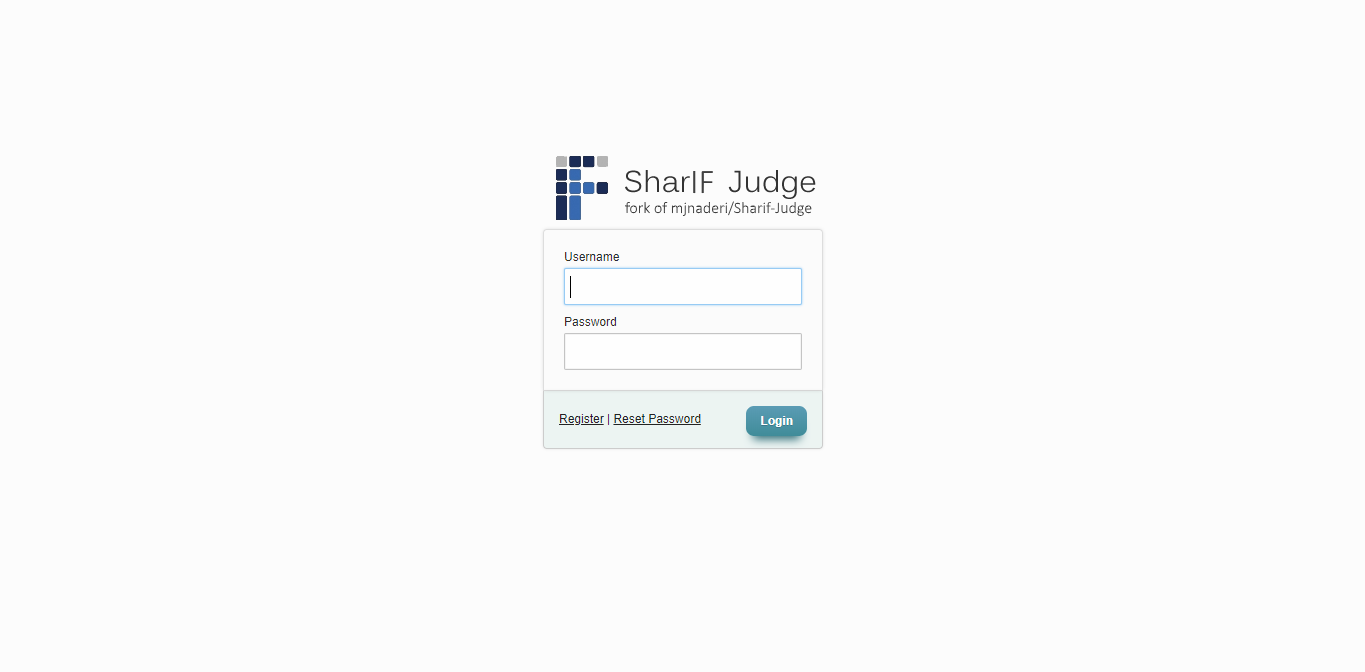
\includegraphics[width=1.0\textwidth]{newlogin}  
		\caption[Tampilan Halaman Login]{Tampilan Halaman Login} 
		\label{fig:newlogin} 
	\end{figure}
	
	\begin{figure}[H]
		\centering  
		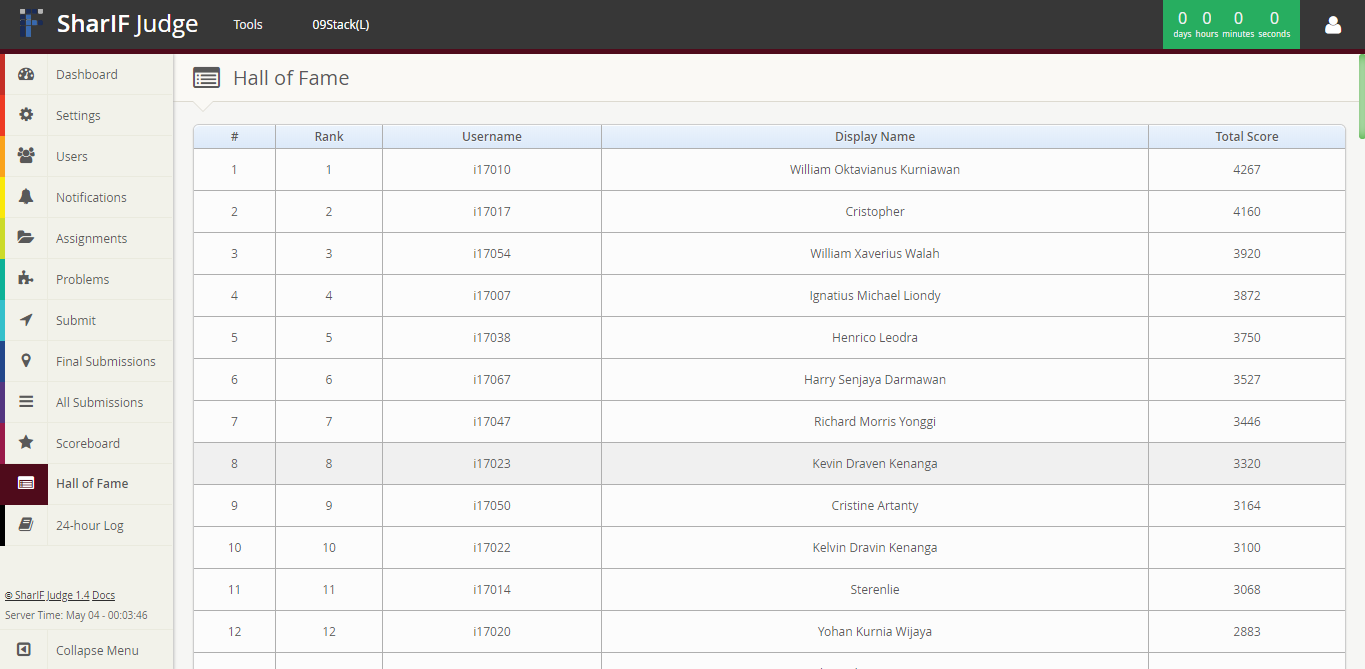
\includegraphics[width=1.0\textwidth]{newhof}  
		\caption[Tampilan Halaman Hall of Fame]{Tampilan Halaman Hall of Fame} 
		\label{fig:newhof} 
	\end{figure}

	\begin{figure}[H]
		\centering  
		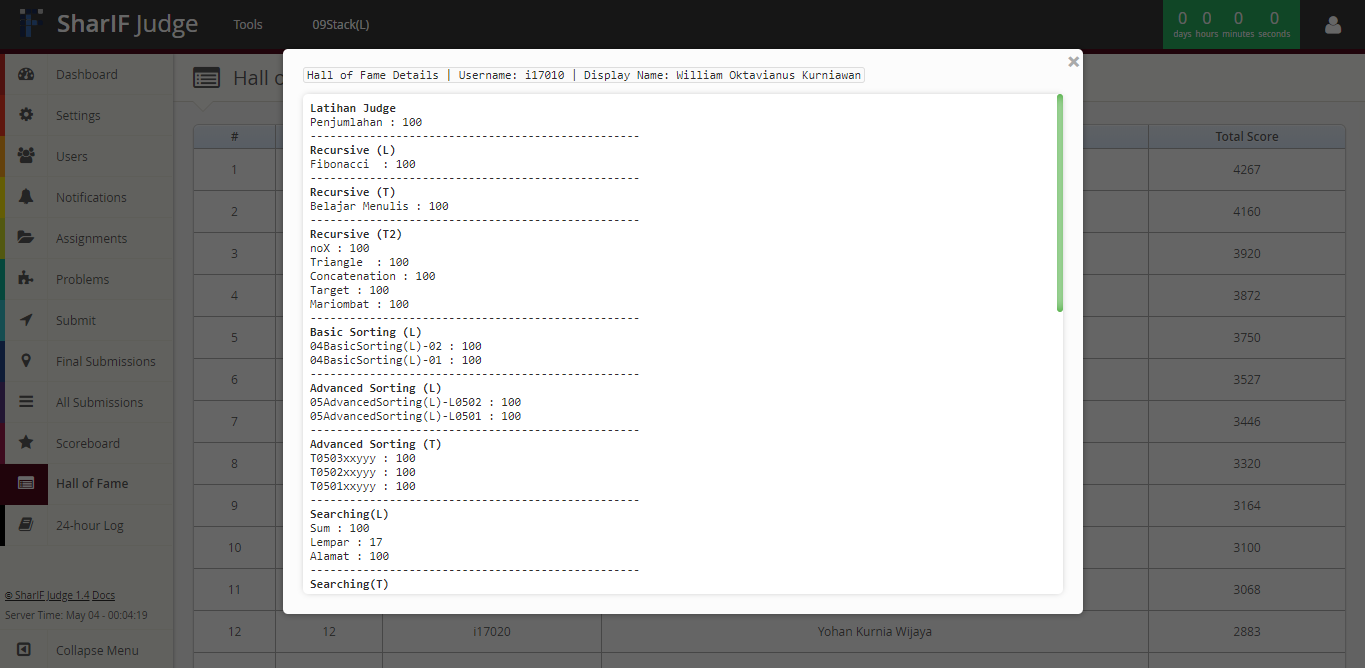
\includegraphics[width=1.0\textwidth]{newhofdetail}  
		\caption[Tampilan Detail dari Hall of Fame]{Tampilan Detail dari Hall of Fame} 
		\label{fig:newhofdetail} 
	\end{figure}

	\begin{figure}[H]
		\centering  
		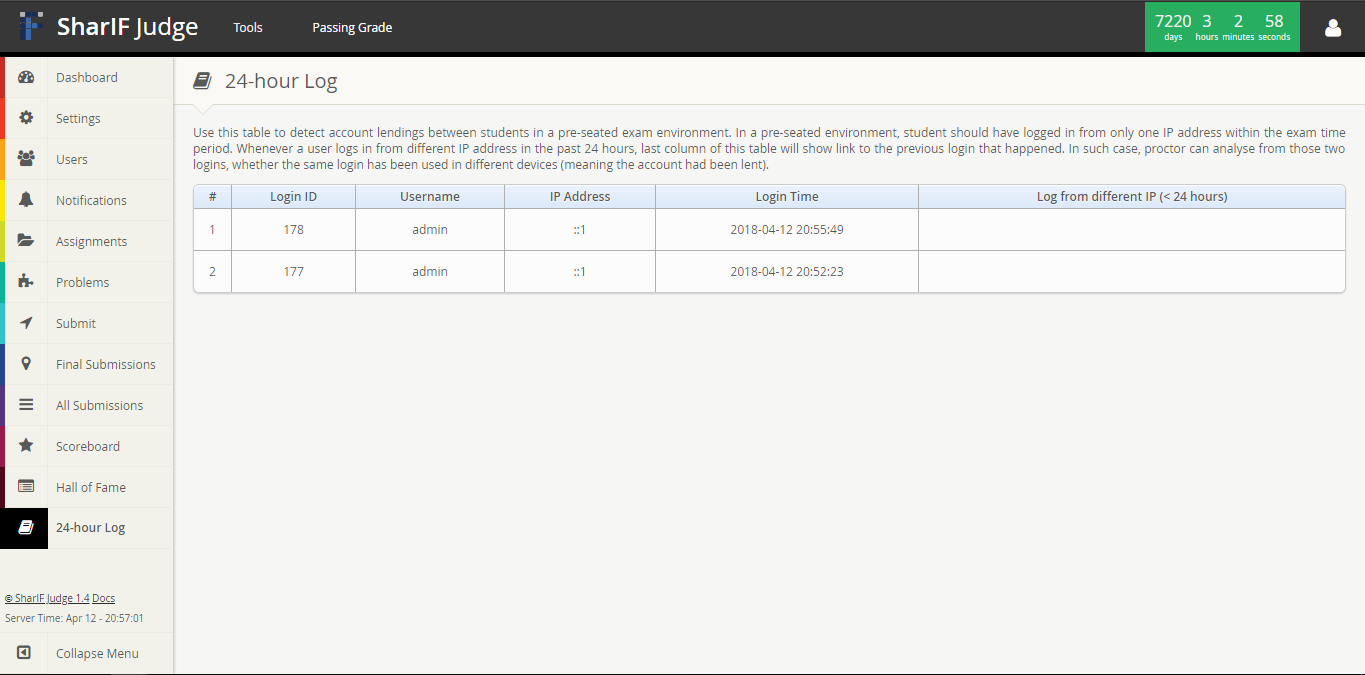
\includegraphics[width=1.0\textwidth]{newlogs}  
		\caption[Tampilan Halaman Logs]{Tampilan Halaman Logs} 
		\label{fig:newlogs} 
	\end{figure}

	\begin{figure}[H]
		\centering  
		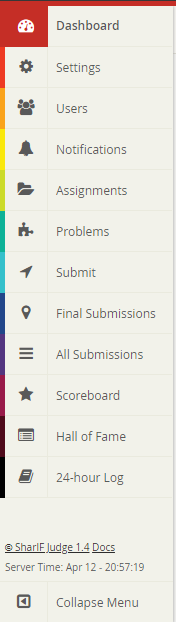
\includegraphics[scale=0.7]{sidemenu}  
		\caption[Tampilan Side Menu]{Tampilan Side Menu} 
		\label{fig:sidemenu} 
	\end{figure}
\end{enumerate}

\section{Pengujian Fungsional}
Pengujian fungsional bertujuan untuk memastikan bahwa perangkat lunak dapat berfungsi sebagaimana mestinya. Jika fungsi yang telah diimplementasi tidak berjalan dengan baik, maka perangkat lunak masih memiliki kekurangan.
	\subsection{Mengunduh Soal (deskripsi \& PDF) yang Telah Dibatasi}
	Hasil yang diharapkan dari pengujian fungsi ini adalah soal dapat dibatasi sesuai dengan ketentuan yang telah dirancang pada \hyperref[chap:batassoal]{sub bab 4.3}. Pengujian dimulai dengan membuat empat buah \textit{assignment}.
	\begin{figure}[H]
		\centering  
		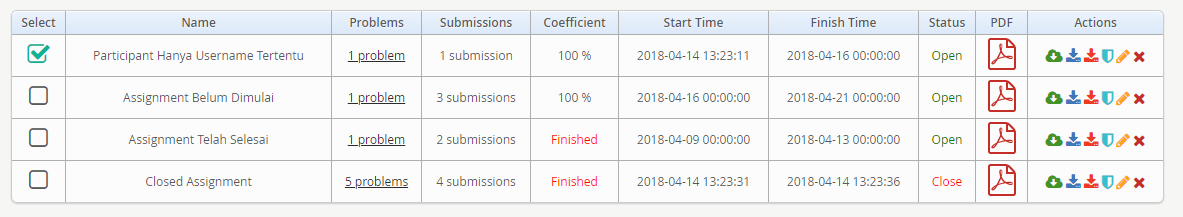
\includegraphics[width=1.0\textwidth]{/pengujian/batasisoal/listassignment}  
		\caption[Empat Buah \textit{Assignment} yang Dibuat]{Empat Buah \textit{Assignment} yang Dibuat} 
		\label{fig:listassignment} 
	\end{figure}
	
	\textit{Assignment} dengan nama "\textit{Participant} Hanya \textit{Username} Tertentu", merupakan \textit{assignment} yang dikhususkan untuk peserta tertentu. \textit{Assignment} dengan nama "\textit{Assignment} Belum Mulai", merupakan \textit{assignment} yang belum dimulai. \textit{Assignment} dengan nama "\textit{Assignment} Telah Selesai", merupakan \textit{assignment} yang waktu pengumpulannya telah habis. \textit{Assignment} dengan nama "\textit{Closed Assignment}", merupakan \textit{assignment} yang memiliki status \textit{close}. \\
	
	Jika peserta yang tidak terdaftar sebagai \textit{participant}, mencoba untuk mengunduh \textit{assignment} dengan nama "\textit{Participant} Hanya \textit{Username} Tertentu", maka muncul pesan \textit{error "You are not registered for submitting."} seperti \hyperref[fig:np]{Gambar 5.7} 
	\begin{figure}[H]
		\centering  
		
\includegraphics[width=1.0\textwidth]{/pengujian/batasisoal/np}  
		\caption[Pesan \textit{Error "You are not registered for submitting."}]{Pesan \textit{Error "You are not registered for submitting."}} 
		\label{fig:np} 
	\end{figure}

	Jika peserta mencoba untuk mengunduh \textit{assignment} dengan nama "\textit{Assignment} Belum Mulai", maka muncul pesan \textit{error "Selected assignment has not started."} seperti \hyperref[fig:ns]{Gambar 5.8} 
	\begin{figure}[H]
		\centering  
		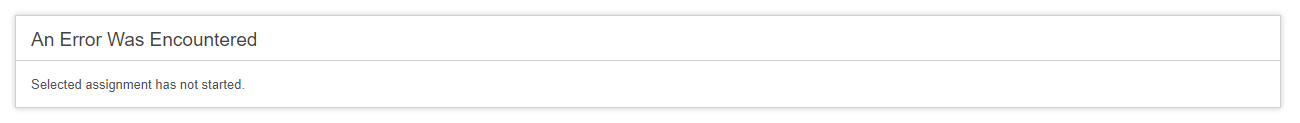
\includegraphics[width=1.0\textwidth]{/pengujian/batasisoal/ns}  
		\caption[Pesan \textit{Error "Selected assignment has not started."}]{Pesan \textit{Error "Selected assignment has not started."}} 
		\label{fig:ns} 
	\end{figure}

	Jika peserta mencoba untuk mengunduh \textit{assignment} dengan nama "\textit{Assignment} Telah Selesai", maka muncul pesan \textit{error "Selected assignment has finished."} seperti \hyperref[fig:f]{Gambar 5.9} 
	\begin{figure}[H]
		\centering  
		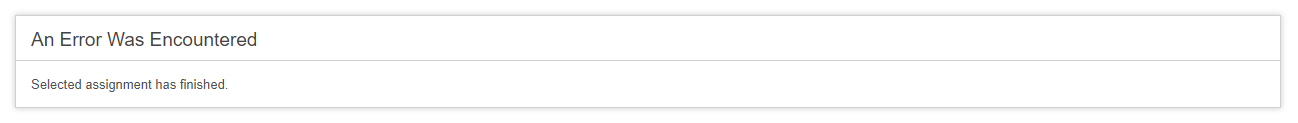
\includegraphics[width=1.0\textwidth]{/pengujian/batasisoal/f}  
		\caption[Pesan\textit{ Error "Selected assignment has finished."}]{Pesan \textit{Error "Selected assignment has finished."}} 
		\label{fig:f} 
	\end{figure}

	Jika peserta mencoba untuk mengunduh \textit{assignment} dengan nama "\textit{Closed Assignment}", maka muncul pesan \textit{error "Selected assignment has been closed."} seperti \hyperref[fig:c]{Gambar 5.10} 
	\begin{figure}[H]
		\centering  
		
\includegraphics[width=1.0\textwidth]{/pengujian/batasisoal/c}  
		\caption[Pesan \textit{Error "Selected assignment has been closed."}]{Pesan \textit{Error "Selected assignment has been closed."}} 
		\label{fig:c} 
	\end{figure}

	\subsection{Membuat \textit{Assignment} yang Menerima \textit{File} dengan Ekstensi TXT}
	Hasil yang diharapkan dari pengujian fungsi ini adalah dosen dapat membuat \textit{assignment} yang bisa menerima \textit{file} dengan ekstensi TXT dan para peserta bisa mengumpulkan file dengan ekstensi TXT ke \textit{assignment} tersebut. Pengujian dimulai dengan membuat \textit{assignment} yang bersifat "\textit{Upload Only}" dan menambahkan '\textit{txt}' pada \textit{text field Allowed Language}.
	\begin{figure}[H]
		\centering  
		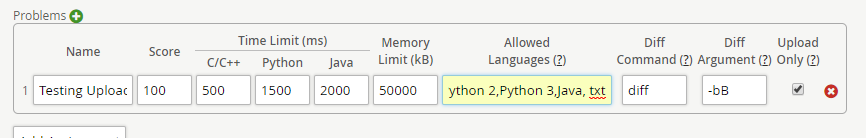
\includegraphics[width=1.0\textwidth]{/pengujian/uploadtxt/uploadtxt}  
		\caption[Pembuatan \textit{Assignment} Upload TXT]{Pembuatan \textit{Assignment} Upload TXT} 
		\label{fig:uploadtxt} 
	\end{figure}
	
	Setelah \textit{assignment} berhasil dibuat, selanjutnya dicoba untuk mengumpulkan \textit{file} dengan ekstensi TXT pada halaman \textit{Submit} seperti \hyperref[fig:submittxt]{Gambar 5.12}. Jika berhasil mengumpulkan \textit{file} TXT, maka peserta langsung diarahkan ke halaman \textit{All Submission} seperti \hyperref[fig:resultttxt]{Gambar 5.13}
	
	\begin{figure}[H]
		\centering  
		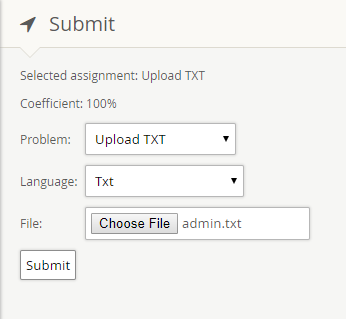
\includegraphics[scale=0.5]{/pengujian/uploadtxt/submittxt}  
		\caption[\textit{Submit File} TXT]{\textit{Submit File} TXT} 
		\label{fig:submittxt} 
	\end{figure}

	\begin{figure}[H]
		\centering  
		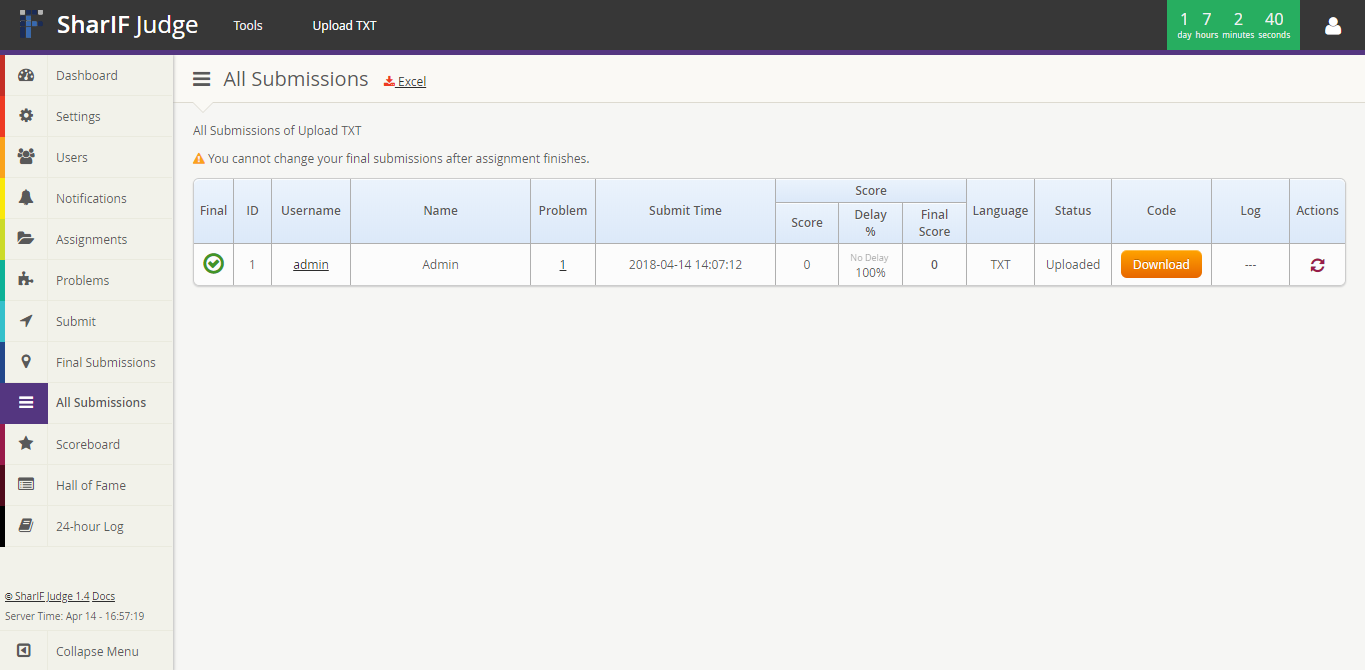
\includegraphics[width=1.0\textwidth]{/pengujian/uploadtxt/resulttxt}  
		\caption[Halaman \textit{All Submission} setelah Mengumpulkan \textit{File} TXT]{Halaman \textit{All Submission} setelah Mengumpulkan \textit{File} TXT} 
		\label{fig:resultttxt} 
	\end{figure}

	Pengujian dilanjutkan dengan mengunduh dan mencocokan isi dari \textit{file} TXT yang baru saja dikumpulkan. Jika isi dari \textit{file} TXT hasil unduh sama dengan \textit{file} TXT utama, maka fitur ini dapat berjalan dengan baik. \hyperref[fig:resultttxt]{Gambar 5.14} merupakan isi dari \textit{file} TXT yang dikumpulkan dan \hyperref[fig:resultttxt]{Gambar 5.15} isi dari \textit{file} TXT utama.
	
	\begin{figure}[H]
		\centering  
		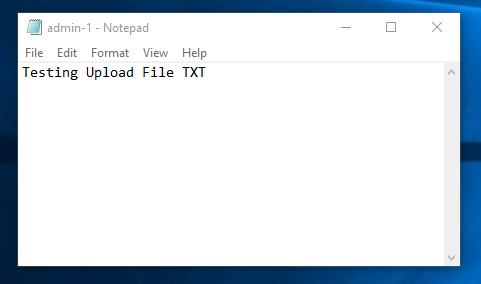
\includegraphics[scale=0.5]{/pengujian/uploadtxt/fileunduh}  
		\caption[\textit{File} TXT Hasil Unduh]{\textit{File} TXT Hasil Unduh} 
		\label{fig:fileunduh} 
	\end{figure}
	
	\begin{figure}[H]
		\centering  
		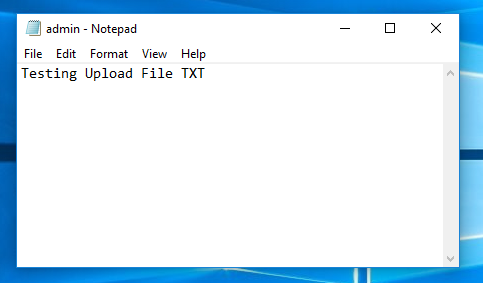
\includegraphics[scale=0.5]{/pengujian/uploadtxt/fileutama}  
		\caption[File TXT Utama]{File TXT Utama} 
		\label{fig:fileutama} 
	\end{figure}

	\subsection{Mengakses Halaman \textit{24-hour Logs}}
	Hasil yang diharapkan dari pengujian fungsi ini adalah halaman \textit{24-hour Logs} dapat menampilkan seluruh aktivitas \textit{login} dari pengguna. Pengujian dimulai dari \textit{login} menggunakan \textit{username} dengan \textit{role admin}. Setelah berhasil \textit{login}, akses halaman \textit{24-hour Logs} yang terletak di paling bawah \textit{side menu}. Halaman \textit{24-hour Logs} tampil seperti \hyperref[fig:logs]{Gambar 5.16}
	\begin{figure}[H]
		\centering  
		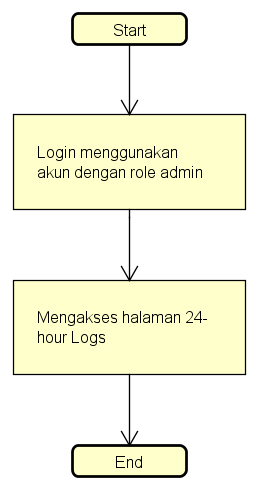
\includegraphics[width=1.0\textwidth]{/pengujian/logs/logs}  
		\caption[Halaman \textit{24-hour Logs} yang Tampil]{Halaman \textit{24-hour Logs} yang Tampil} 
		\label{fig:logs} 
	\end{figure}

	Pengujian dilanjutkan dengan mencoba \textit{login} menggunakan \textit{username} yang sama namun menggunakan \textit{ip address} yang berbeda. Hasil yang diharapkan adalah halaman \textit{24-hour Logs} dapat mencatat dan menampilkan Login ID yang menggunakan \textit{ip address berbeda}.
	\begin{figure}[H]
		\centering  
		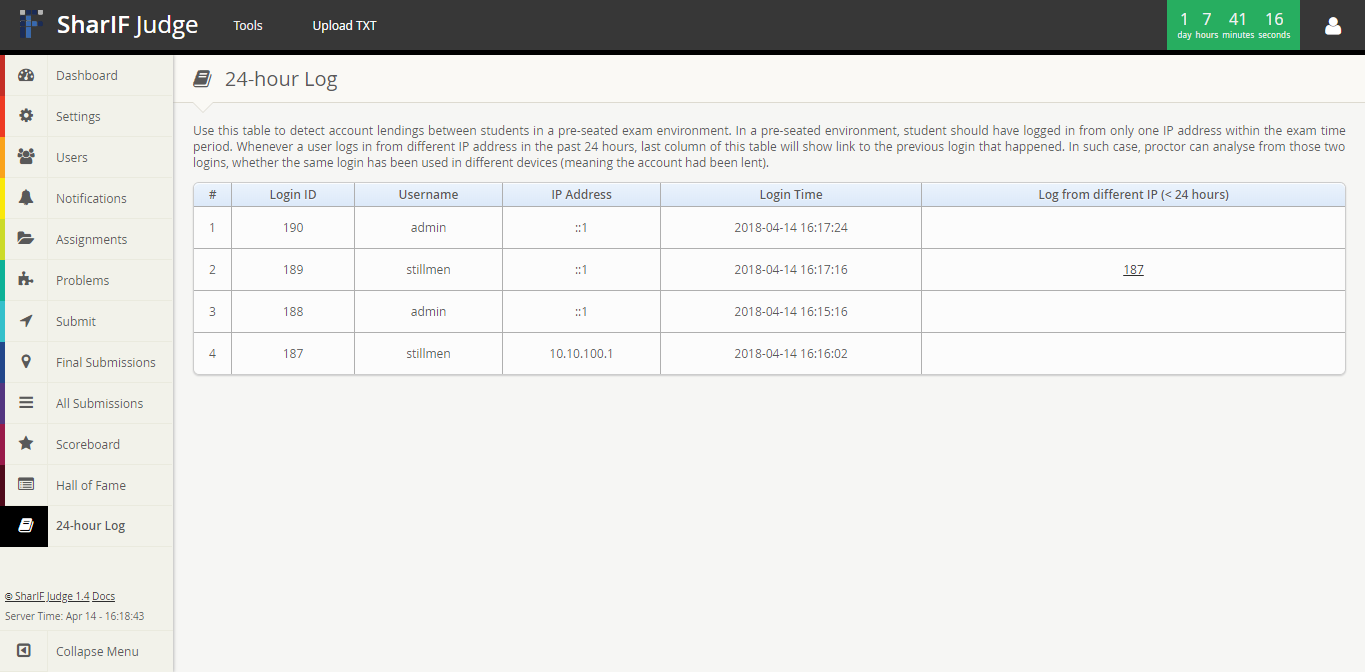
\includegraphics[width=1.0\textwidth]{/pengujian/logs/logs1}  
		\caption[Halaman \textit{24-hour Logs} Mencatat Aktivitas \textit{Login} Pengguna]{Halaman \textit{24-hour Logs} Mencatat Aktivitas \textit{Login} Pengguna} 
		\label{fig:logs1} 
	\end{figure}
	Terlihat pada \hyperref[fig:logs1]{Gambar 5.17}, \textit{username} stillmen pertama kali \textit{login} menggunakan \textit{ip address} 10.10.100.1 (baris 4). Setelah mencoba untuk \textit{login} menggunakan \textit{ip address} yang berbeda, halaman \textit{24-hour Logs} dapat mencatat dan menampilkan \textit{Login ID} dari \textit{username} stillmen (baris 2).